\chapter{Misure con oscilloscopio digitale su amplificatore operazionale in configurazione catena chiusa}
\label{chap:terza_prova}

\section*{Obiettivo}
L'obiettivo della terza esperienza di laboratorio è quello di valutare la frequenza di taglio e il guadagno di un amplificatore operazionale in configurazione a \emph{catena chiusa} (closed-loop) al fine di effettuare il tracciamento della risposta in frequenza del circuito integrato in questione.

\section{L'amplificatore operazionale µA741}
L'amplificatore operazionale (OP-AMP) è un dispositivo attivo, dotato cioè di alimentazione, in grado  di amplificare i segnali in ingresso. Durante l'esperienza è stato usato l'OP-AMP µA471, provvisto dei seguenti pin:
\begin{itemize}
    \item V\textsubscript{+} morsetto non invertente
    \item V\textsubscript{-} morsetto invertente
    \item V\textsubscript{o} pin d'uscita
    \item +V\textsubscript{cc} e -V\textsubscript{cc} pin per l'alimentazione in continua
    \item due pin per la compensazione dell'offset
\end{itemize}

\begin{figure}
    \centering
    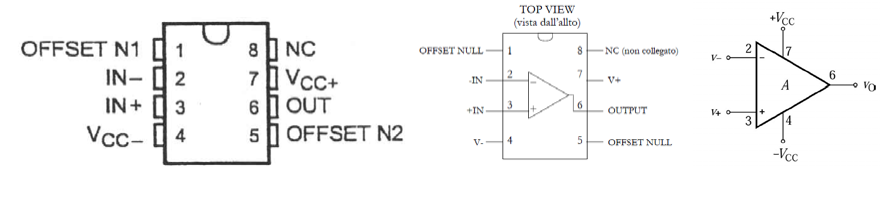
\includegraphics[width=1\linewidth]{Relazione//media/uA741.png}
    \caption{Piedinatura e schema interno del $\mu$A741}
    \label{fig:Piedinatura e schema interno del uA741}
\end{figure}
\FloatBarrier
\section{Caratterizzazione µA741 in catena chiusa}
Dalle specifiche del µA741, si può osservare che questo circuito integrato richiede un’alimentazione duale compresa tra ±9V e ±15V. In questa prova, per l'integrato, attraverso un generatore di compensazione, è stata impostata un'alimentazione di ±12V con l'uso dei tasti +25 e -25 e successivamente effettuando la regolazione con la manopola presente sul generatore.

\subsubsection{Gain Bandwidth Product (GBWP) – Prodotto banda-guadagno}
Il GBWP di un amplificatore operazionale è il prodotto tra il modulo del suo guadagno ad anello aperto e la frequenza di taglio a 3 dB. In pratica, è la frequenza a cui il guadagno di tensione ad anello aperto si riduce al valore unitario. Questo parametro (caratteristico per ciascun amplificatore), essendo costante a qualsiasi
frequenza, permette di determinare il massimo guadagno ottenibile da uno strumento ad una determinata frequenza, e viceversa. Dal grafico disponibile sul datasheet dell’amplificatore, Figura \ref{fig:Diagramma Avd vs Frequenza},  si osserva che ad un guadagno di 0 dB ad anello aperto corrisponde una frequenza pari ad 1 MHz.
Pertanto si può determinare la banda passante (B) e la frequenza di taglio teorica (f\textsubscript{c}):

\[f_c=B=\frac{GBWP}{|A|}\]
\begin{figure}
    \centering
    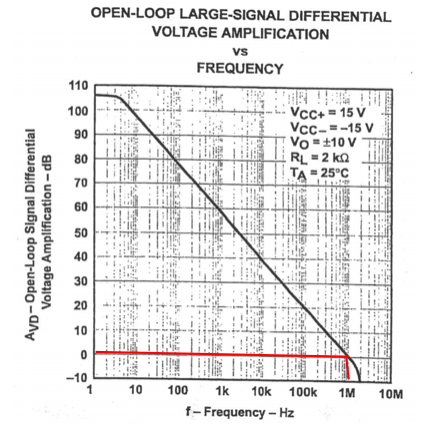
\includegraphics[width=0.5\linewidth]{diagrammaOLvsFreq_uA741.png}
    \caption{Diagramma $A_{VD}$ vs Frequenza}
    \label{fig:Diagramma Avd vs Frequenza}
\end{figure}
\FloatBarrier

\subsection{Tensione di offset e compensazione}
Idealmente, un amplificatore differenziale alimentato con una tensione duale e con ingressi collegati entrambi a massa, dovrebbe fornire in uscita una tensione pari a 0 V. In realtà, invece, esistono sempre delle dissimmetrie interne di funzionamento che danno origine ad una piccola tensione d’uscita, cioè la “tensione di offset”. Pertanto, data la non idealità dell'OP-AMP, i pin 1 e 5 devono essere regolati, facendo riferimento alla Figura \ref{fig:Piedinatura e schema interno del uA741}. Sperimentalmente, l’effetto dell’offset può essere osservato effettuando i seguenti passaggi:

\begin{enumerate}
    \item Alimentando l’operazionale e non fornendo alcun segnale agli ingressi;
    \item  Sull’oscilloscopio, serve visualizzare solo il canale al quale è collegato l’uscita dell’amplificatore operazionale.
    \item  Il segnale è in continua, con sovrapposto un segnale di rumore (Figura \ref{fig:tensioneOffset}): per questo, è opportuno eseguire una misura mediata della tensione efficace (\textit{Misura RMS}), andando a selezionare prima il tasto \textit{Mesure}.
    \item  Per compensare l’offset in modo da riportare a 0 V la tensione in uscita, è necessario collegare fra i due pin interessati (offset o balance), un trimmer il cui cursore risulti collegato alla tensione di alimentazione oppure a massa.
    \item Regolare tale trimmer fino a rilevare in uscita una tensione nulla (Figura \ref{fig:azzeramentoOffset}). 
\end{enumerate}

Operativamente, per annullare l’offset, si utilizza il trimmer già presente sul circuito fornito durante l’esercitazione: tramite un cacciavite, si ruota la vite presente fin quando non vengono letti valori dell’ordine di pochi µV.
Nel caso dell'esperienza, è stato fissato un valore pari a:

\[V_{rms}=866,4 \mu V\]
\FloatBarrier
\begin{figure}
    \centering
    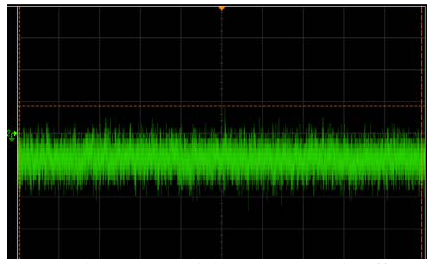
\includegraphics[width=0.5\linewidth]{Relazione//media/tensioneOffest.png}
    \caption{Tensione di offest vista sull'scilloscopio}
    \label{fig:tensioneOffset}
\end{figure}
\begin{figure}
    \centering
    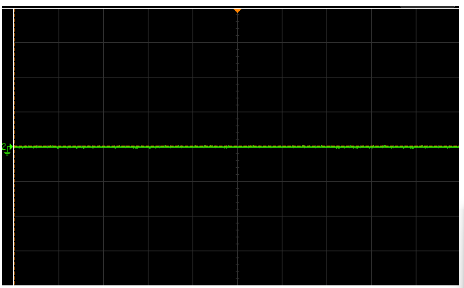
\includegraphics[width=0.5\linewidth]{Relazione//media/azzeramentoOffset.png}
    \caption{Azzeramento dell'offset visto sull'oscilloscopio}
    \label{fig:azzeramentoOffset}
\end{figure}
\FloatBarrier
\subsection{Misure di guadagno e frequenza di taglio in catena chiusa}

Il circuito nella configurazione “a catena chiusa” è stato realizzato direttamente su una scheda elettronica, di cui la schematizzazione è in Figura \ref{fig:schemaCatenaChiusa}:

\begin{figure}
    \centering
    \includegraphics[width=1\linewidth]{circuitoIntegrato_uA741.png}
    \caption{Schema circuitale della configurazione in catena chiusa}
    \label{fig:schemaCatenaChiusa}
\end{figure}

\FloatBarrier
Nel circuito di interesse, la resistenza \(R_6\) (tra ingresso invertente dell’amplificatore ed il pin di uscita) ed \(R_{12}\) (tra ingresso invertente dell’amplificatore ed ingresso dell’amplificatore) determinano il guadagno in catena chiusa dell’amplificatore, che vale:

\[A_{Teorico}=-\frac{R_6}{R_{12}}=-\frac{22 k\Omega}{1 k\Omega}=-22\]

La resistenza \(R_{14}\) posta tra l’ingresso non invertente e massa serve per non collegare direttamente l’ingresso non invertente a massa, ma ad un valore di resistenza prossimo a quello dell’ingresso invertente. La resistenza variabile \(R_{18}\) (da 10 k\(\Omega\)) è di tipo multi-giro e serve a compensare il valore di tensione di offset. Dopo aver ridotto l’offset, e stimato il segnale di ingresso in ampiezza e frequenza, per mezzo del generatore di funzioni si fornisce in ingresso al circuito un segnale sinusoidale. Partendo da questo valore di ampiezza, si varia l’ampiezza del segnale (aumentandola o diminuendola) fino ad ottenere la massima tensione d’uscita picco-picco. Se l’ampiezza del segnale supera il valore massimo, l’amplificatore raggiunge la regione di saturazione.
Per la valutazione sperimentale del guadagno, serve effettuare la stima delle tensioni picco-picco \(V_{o,pp}\)
e \(V_{i, pp}\) attraverso l'utilizzo dell'oscilloscopio. Da queste due stime si è ottenuto:

\[V_{o,pp}=4,125V\]

\[V_{i, pp}=190,6mV\]
Da cui:

\[A=-\frac{V_{o,pp}}{V_{i, pp}}=-21,6\]
Andando a determinare quanto vale A, in corrispondenza della frequenza di taglio \(f_c\), tale per cui si ha un'attenuazione di 3dB, segue che:

\[A_{-3dB}=\frac{A}{\sqrt{2}}=-15,27\]
Infine, è possibile calcolare il valore della tensione di uscita in corrispondenza della frequenza di
taglio, facendo uso della relazione:

\[V_o=A_{-3dB} \cdot V_i=2,91V_{pp}\]
Per la valutazione sperimentale della frequenza di taglio, si impostano i due cursori orizzontali dell’oscilloscopio in corrispondenza di questo valore di tensione. Si procede quindi a variare la frequenza del segnale fino a che il segnale in uscita visualizzato sull’oscilloscopio non risulta tangente ai due cursori orizzontali. In corrispondenza della frequenza di taglio, si può notare che il segnale in uscita è distorto (segnale triangolare) e che il valore di frequenza trovato è diverso dal valore teorico. Questo succede perché si sta lavorando con un segnale di ingresso con ampiezza massima. Per evitare questo effetto, è necessario ridurre l’ampiezza del segnale, ricalcolare il nuovo valore di attenuazione a 3dB e, quindi, stimare la frequenza di taglio. In questo caso, si è trovato che \(f_c=33kHz\).
Per verificare quanto detto sopra, la frequenza di taglio teorica \(f_{c_{teorica}}\), si ricava dalla relazione già espressa precedentemente, per cui:

\[f_{c_{teorica}}=\frac{GBWP}{|A|}=45,5kHz\]
\subsection{Misurazioni}



\subsection{Calcolo delle incertezze}
